% !TEX program = xelatex

\documentclass[Chinese,TC,use boldface,simple Names]{beaulivre}
\usepackage{hls_tutorial}

%%================================
%% Main text
%%================================
\begin{document}

\frontmatter

\TitlePage [
    color = { main = forestgreen!75!black, back = forestgreen!10!yellow!30 },
    logo = {
\includegraphics[width=2cm]{logos/vitis_hls.png}}
  ]
  {
    , title     = Vitis~ HLS~ Tutorial~ Step~ by~ Step
    , subtitle  = {
                    \textsc{用 C++ 做硬件设计的黑科技}\\[10pt]
                    \small Xilinx Vivado \texttt{2017.4}\\[-2pt]
                    \small Xilinx Vitis\hspace{\widthof{Vivado}-\widthof{Vitis}} \texttt{2021.2}
                  }
    , author    = 赵舞穹,LEADS
    , date      = {\today{},南京}
  }


\chapter{前言}

  硬件设计好难,从C++使用 Vivado 的高级综合(high level synthesis,HLS)工具也好难。
  我就将我一步一步的踩坑记录在这里。

  记号 \UGvitis{123--456} 和 \UGvivado{123--456}
  分别表示 Vitis High-Level Synthesis User Guide (UG1399, v2021.2)
  和 Vivado Design Suite User Guide: High-Level Synthesis (UG902, v2017.4)
  中对应的页码。

\tableofcontents

\mainmatter

\part{准备工作}
\parttext{“磨刀不误砍柴工”,正式研究 HLS 设计之前应该有一定的理论知识。最直接的问题是软件及环境的配置需要准备完善,否则各种报错实在令人头秃。}

\chapter{理论知识}

\chapter{软件环境}

  \section{软件版本}

    我主要使用 Vitis 2021.2 版本进行工作,
    同时由于课题组之前常用 2017.4 并且其软件大小相对较小,我也将兼顾对 2017.4 版本的兼容。
    下载对应版本可以自行前往 Xilinx 官网。
    安装完成后可以导入对应的 License 完成激活。

    \begin{table}[htbp]
      \caption{版本对比}
      \label{tab:hls_version}
      \renewcommand*{\arraystretch}{1.3}
      \begin{tabularx}{\linewidth}{>{\bfseries\arraybackslash}cYY}
        \toprule
        & \textbf{\color{maintheme}Vitis HLS 2021.2} & \textbf{\color{maintheme}Vivado HLS 2017.4} \\
        \midrule
        Logo & 
\includegraphics[height=15mm]{logos/vitis_hls.png} & 
\includegraphics[height=15mm]{logos/vivado_hls.jpeg} \\ \hline
        Windows 支持版本 & 10 \& 11 & 7 \& 10 \& (11) \\ \hline
        Ubuntu 支持版本 & 16 \& 18 \& 20 & 16 \\ \hline
        GCC 版本 & 6.2.0 & 4.6.3 \\ \hline
        C++ 标准 & C++14 & C++98 \\ \hline
        套装软件大小(Ubuntu) & 120.1G & 37.1G \\
        \bottomrule
      \end{tabularx}
    \end{table}

    两个版本 HLS 工具的主要区别在\cref{tab:hls_version} 中给出,
    可以发现,总体来说 Vitis 2021.2 会提供更好的支持(例如可以使用更新的 C++ 语法),并且会有更快的速度。
    不过相较于 Vivado 2017.4 软件大小会大很多,如果之前已经有 Vivado 2017.4 也可以不需要使用 Vitis 2021.2。

  \section{操作系统}

    \subsection{Windows}

      在 Windows 上运行 Vivado 2017.4 以及其 Vivado HLS 都是非常丝滑的,Vivado 支持 Windows 7 及以上版本。
      虽然官方文档没有指出对于 Windows 11 的支持性,但由于 Windows 11 与 Windows 10 的相似性,
      Windows 11 在我目前的测试下仍然没有问题。
      (不过 Vivado 2017.4 非 100\% 屏幕缩放会导致的模糊问题还没有得到解决,只能自己再忍一忍,或者跑路去 Linux,至少 Ubuntu 20 屏幕看上去就没有磨砂质感的界面了。
      Vivado HLS 的界面效果是都没有问题的。)

      如果使用 Vitis 2021.2 体验就会比 Vivado 2017.4 还要丝滑,Windows 上也解决了界面模糊的问题。

      \begin{tip}
        我使用的版本是 Windows 11 Professional。
      \end{tip}

    \subsection{Linux}

      Linux 上使用 Vivado 2017.4 和 Vivado HLS 2017.4 相对 Windows 就会痛苦不少,主要体现在以下几个方面:
      \begin{enumerate}
        \item Linux 版本对于环境依赖性强,在安装和使用的过程中会使用到不少的包,例如 \texttt{libtinfo5} 等;
        \item HLS 环境的 C 及 C++ 的 include 路径会包括用户系统中 C 或 C++ 编译器的默认路径,造成头文件和 HLS 提供的编译器版本不匹配;
        \item Vivado 2017.4 支持的 Linux 系统版本较老,例如 Ubuntu 只正式支持 16。
      \end{enumerate}

      \begin{warning}
        意识到了上述的几个问题之后,还是不建议使用 Linux 使用 Vivado HLS 2017.4 相关工作,除非你对于 Linux 或 Unix 环境的配置绝对在行。
      \end{warning}

      如果想要尝试使用 Linux 版本的 Vivado 2017.4 的话,有如下几个技巧:
      \begin{itemize}
        \item 安装时缺包可以参考\href{https://support.xilinx.com/s/article/63794?language=en_US}{官方文章};
        \item HLS 工具选择 C 仿真编译器在 GCC 和 Clang 之间切换,可能其中的某一个可以成功。(Ubuntu 20 上 Clang 可以完成简单的 C 仿真,综合都是可以的。但是在 C 与 RTL 的联合仿真中两个编译器都失败了。)
        \item 如果仍然有问题,还是需要安装 Vitis 2021.2。硬盘空间不够甚至可以选择安装在移动硬内。
      \end{itemize}

      使用 Vitis 2021.2 体验就比较好,因为 Vitis 2021.2 支持 Ubuntu 18 和 Ubuntu 20。
      具体信息可以参考 Xilinx 网站。

      \begin{tip}
        我使用的发行版是 Ubuntu 20.04.3 LTS。
      \end{tip}

\part{快速入门}
\parttext{“千里之行,始于足下”,首先从例子出发,完整的感受 HLS 设计的流程,在这之后我们再去深入探讨 HLS 中的众多技巧。}

\chapter{Hello World}\index{Hello World}

  \section{案例目标}

    在这个例子中,我们遵从 Hello World 的经典历史传承,使用 C++ 运用 HLS 工具设计一个 \texttt{helloworld} 模块并将其封装成 IP 核,再使用 Verilog 完成其波形测试。
    用 C++ 而不是纯 C 的原因是 C++ 在 C 的基础上增添了许多简便的操作,
    这将进一步简化我们硬件设计的难度。

    在开始工作之前,先介绍 HLS 的\href{https://docs.xilinx.com/v/u/2017.4-English/ug902-vivado-high-level-synthesis}{官方文档},
    虽然官方文档的长度令人害怕,但是像是一本工具书,
    可以查看我们所需要的一些设置。(不会吧,不会还有人不知道这个\href{https://docs.xilinx.com/v/u/2017.4-English/ug902-vivado-high-level-synthesis}{官方文档}四个字其实带超链接的吧。)

    \begin{definition}[HLS 操作步骤缩写定义]
      为了描述简便,我们给出如下一些缩写定义:
      \begin{itemize}
        \item \index{CSim}\textbf{CSim}:C 仿真(也包括 C++ 仿真),C Simulation;
        \item \index{Syn}\textbf{Syn}:综合,Synthesis;
        \item \index{CoSim}\textbf{CoSim}:C 与 RTL 联合仿真,C/RTL Co-Simulation;
        \item \index{Exp}\textbf{Exp}:导出(例如导出为 Verilog IP 核),Export。
      \end{itemize}
      因此,整个 HLS 操作步骤可以被描述为
      \[
        \text{CSim}\longrightarrow\text{Syn}\longrightarrow\text{CoSim}\longrightarrow\text{Exp}.
      \]
    \end{definition}

    以下例子使用 Vivado 2017.4,Vitis 2021.2 类似,操作系统为 Windows 11 Professional。

    \begin{tip}
      案例提供在 \url{https://github.com/SEU-LEADS/HLS_Examples},C++ 代码在 \texttt{Basic/helloworld} 文件夹内,Verilog 测试文件在 \texttt{verilog/helloworld} 内。
      
    \end{tip}

  \section{创建项目}

    打开 HLS 工具,进入欢迎(Welcome)界面,如\cref{fig:welcome} 所示。
    \begin{figure}[htbp]
      \centering
      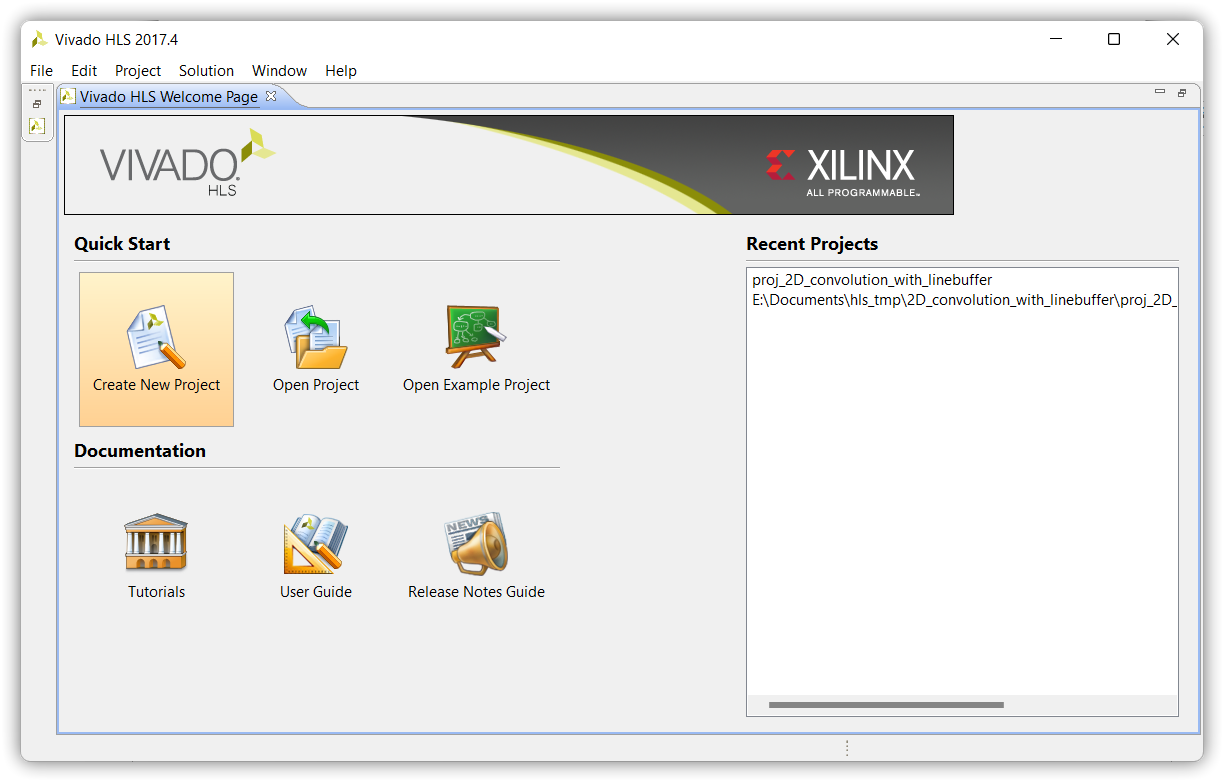
\includegraphics[width=.8\linewidth]{win/helloworld/welcome.png}
      \caption{欢迎界面}
      \label{fig:welcome}
    \end{figure}
    在创建我们需要的 Hello World 之前可以选择
    Open Example Project 查看并仿真、综合提供的示例代码。
    点击 Create New Project 创建新项目,
    可以看到如\cref{fig:new_project} 所示的界面,设置项目的名称和路径,
    项目名称设置为 \texttt{helloworld} 即可。
    需要注意的是项目会创建一个路径下的新文件夹,因此不需要为项目单独创建一个文件夹。
    \begin{warning}
      注意项目路径中不能包含空格。所以尽量也不要在路径中使用中文或其他特殊字符。
    \end{warning}

    接下来两步分别要求添加源代码和测试(testbench)代码,按照要求添加即可。
    此处我们可以先不添加,在创建完项目后单独新建。
    添加源代码时需要设置 top 模块的名称,设置其为 \texttt{helloworld}(此设置后续仍然可以更改)。
    最后,需要设置解决方案(solution)的名称,默认为 \texttt{solution1},我们也不对其进行修改。
    时钟周期(Clock Period)以及不确定度(Uncertainty)可以自行设置,不确定度可以空着使用默认值。
    在这个界面同时需要设置使用的芯片,简单起见,这里就选用了开发版(Board)Virtex-7 VC709 Evaluation Platform,
    这对于目前的例子影响不大,如\cref{fig:init_sol} 所示。
    \begin{figure}[h!]
      \centering
      \subfloat[创建新项目]{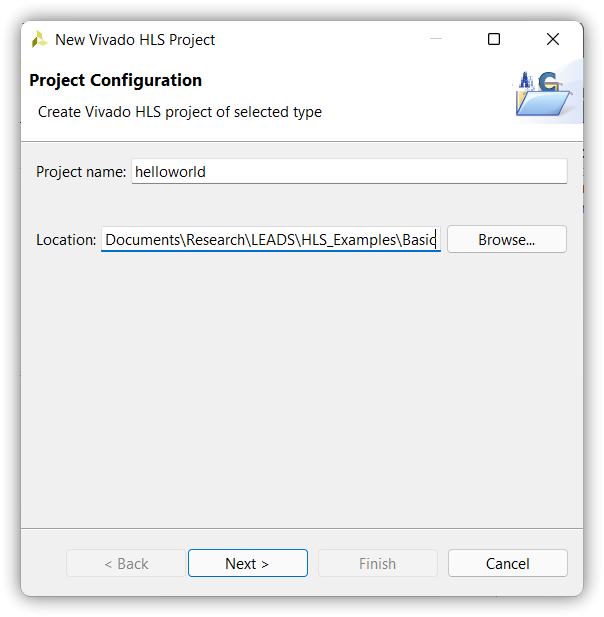
\includegraphics[width=.4\linewidth]{win/helloworld/new_project.png}\label{fig:new_project}}\quad
      \subfloat[设置解决方案等]{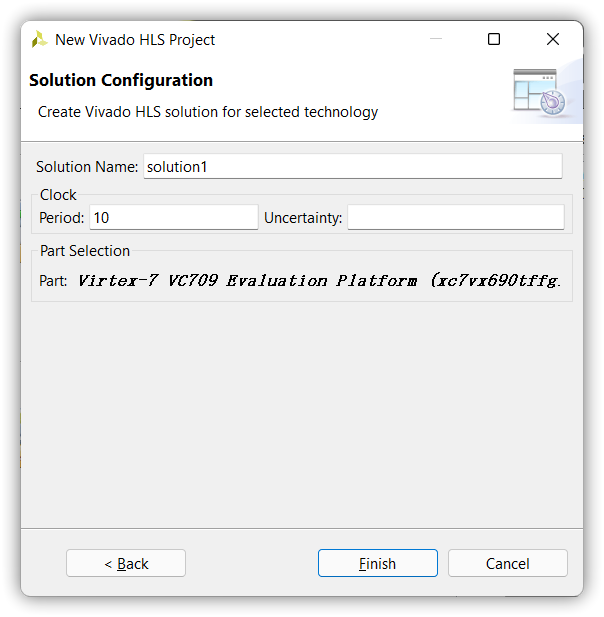
\includegraphics[width=.4\linewidth]{win/helloworld/init_sol.png}\label{fig:init_sol}}
      \caption{创建并设置新项目}
    \end{figure}

  \section{使用 C++ 进行模块设计}

    接着,我们就可以进行 C++ 的 \texttt{helloworld} 模块设计,
    在左侧 Explorer 框的 Includes、Sources 和 Test Bench 中分别添加头文件(\texttt{.h})、源文件(\texttt{.cpp})和测试文件(包括 \texttt{main} 函数的 \texttt{.cpp} 以及其他测试中运用到的文件,例如数据文件 \texttt{.dat} 等)。
    
    此处建议使用其他的文本编辑器编辑代码,这能够提供更加丝滑的 coding 体验,例如
    \begin{figure}[htbp]
      \centering
      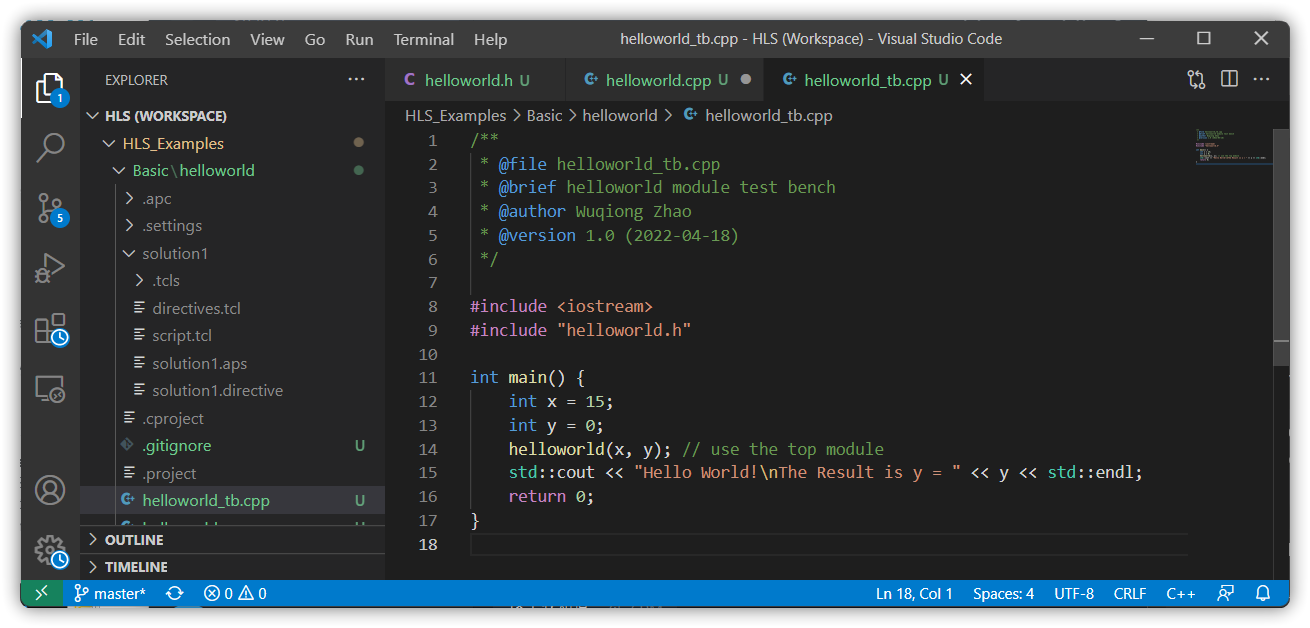
\includegraphics[width=.8\linewidth]{win/helloworld/vscode_edit.png}
      \caption{使用 VS Code 编辑 C++ 代码}
    \end{figure}

    忽略文件信息注释,主要的三个文件代码及解释如下。

    头文件 \texttt{helloworld.h} 申明了函数 \texttt{helloworld},
    这个函数返回值为空(\texttt{void}),
    而是使用了类似 Verilog 的输入输出模式:
    输入为 \texttt{int} 类型的变量 \texttt{a},采用传值的形式,对应 Verilog 中的 \texttt{input};
    输出为 \texttt{int\&} 类型的变量 \texttt{b},采用引用可以对其值进行修改,对应 Verilog 中的 \texttt{output}。
    \begin{warning}
      此处的函数及变量命名为了简便起见(且符合 C++ 命名习惯),没有按照 Verilog 规范进行。
      之后完整的示例中将会规范命名。
    \end{warning}
    \begin{lstlisting}[language=C++, title={helloworld.h}]
#ifndef _HELLOWORLD_H_
#define _HELLOWORLD_H_

/**
 * @brief helloworld module
 * @details right shift a one bit
 * @param a [in] integer
 * @param b [out] the shifted value
 */
void helloworld(int a, int& b);

#endif
    \end{lstlisting}
    
    \texttt{helloworld} 函数的实现则在 \texttt{helloworld.cpp} 中完成,
    内容非常简单,输出的 \texttt{b} 就是输入 \texttt{a} 逻辑右移一位的结果。
    \begin{lstlisting}[language=C++, title={helloworld.cpp}]
#include "helloworld.h"

void helloworld(int a, int& b) {
    b = a >> 1; // right shift one bit
}
    \end{lstlisting}

    函数功能的验证在 \texttt{helloworld\_tb.cpp} 中完成,包括了 \texttt{main} 函数。
    \begin{lstlisting}[language=C++, title={helloworld\_tb.cpp},morekeywords={std,cout,endl}]
#include <iostream>
#include "helloworld.h"

int main() {
    int x = 15;
    int y = 0;
    helloworld(x, y); // use the top module
    std::cout << "Hello World!\nThe Result is y = " << y << std::endl;
    return 0;
}
    \end{lstlisting}

  \section{CSim --- C++ 仿真测试}\index{CSim}

    在上一个步骤完成 C++ 代码的书写,
    可以进行 C Simulation,其对应的按钮图标为“窗口框左下有一个绿三角”,即\cref{fig:C_simulation} 右上角的图标。(Vitis 2021.2 为绿色箭头下拉框 C Simulation。)
    \begin{figure}[htbp]
      \centering
      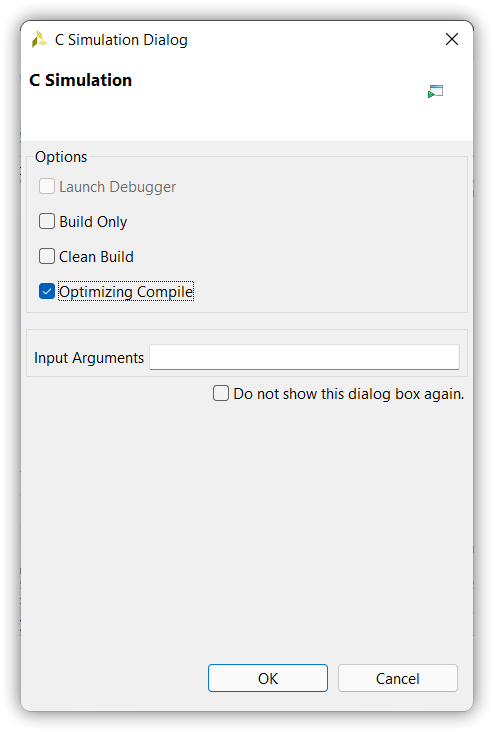
\includegraphics[width=.3\linewidth]{win/helloworld/C_simulation.png}
      \caption{CSim 设置}
      \label{fig:C_simulation}
    \end{figure}

    点击后会弹出\cref{fig:C_simulation} 的设置,四个选项分别表示调试(Debug 模式)、仅编译、清理编译和优化编译(Release 模式)。
    此处我们选择优化编译。
    \begin{tip}[Linux 系统功能(仅限 Vivado 2017.4)]
      如果在 Linux 系统上,还可以选择 C++ 编译器为 GCC 或 Clang。
    \end{tip}
    Input Argument 是 C++ 编译时的命令行选项,例如增加 \texttt{-std=c++03} 可以设置 C++ 编译标准为 C++03。
    如果编译成功,我们会得到如\cref{fig:csim_result} 中的结果,可以看到,输出结果 \texttt{7} 正是我们预期的。
    % 另外可以观察到多出了 \texttt{csim} 文件夹。
    \begin{figure}[htbp]
      \centering
      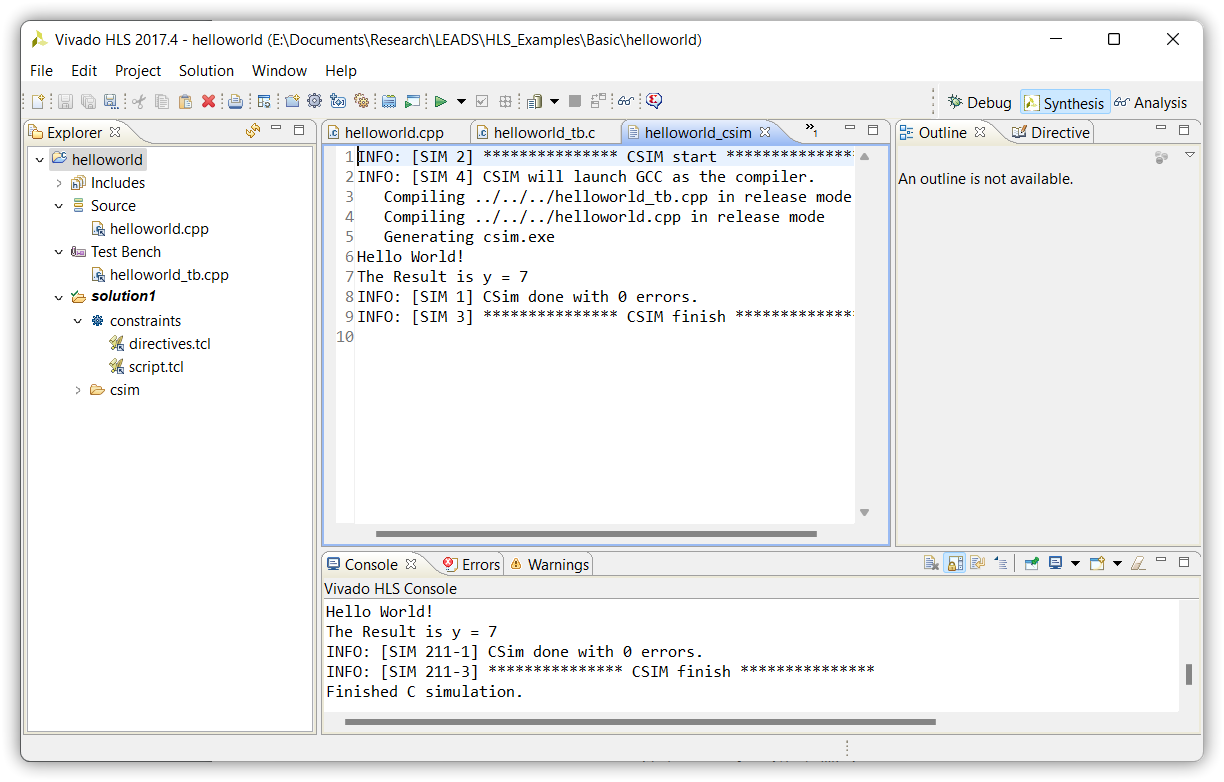
\includegraphics[width=.8\linewidth]{win/helloworld/csim_result.png}
      \caption{CSim 结果}
      \label{fig:csim_result}
    \end{figure}

  \section{Syn --- 综合}\index{Syn}

    完成 C 仿真后,点击 CSim 右边绿箭头进行综合(Vitis 2021.2 为绿色箭头下拉框 C Synthesis),可以得到\cref{fig:syn_result} 中的结果。
    中间页面给出了综合报告,对于各项资源的利用给出了分析。
    另外,点击窗口右上角的 Analysis,可以查看其他例如时序的分析结果。
    \begin{figure}[htbp]
      \centering
      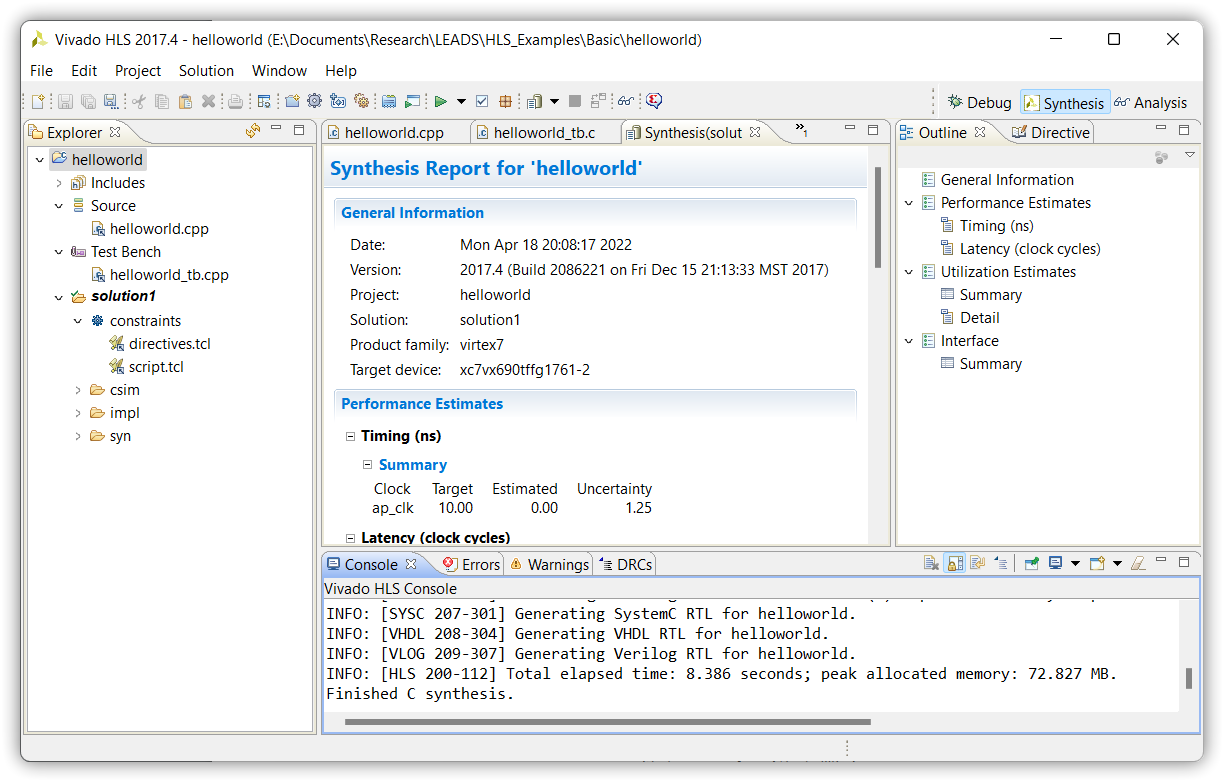
\includegraphics[width=.8\linewidth]{win/helloworld/syn_result.png}
      \caption{Syn 结果}
      \label{fig:syn_result}
    \end{figure}
    \begin{warning}
      Syn 时使用的逻辑与 CSim 和 CoSim 不一样,所以经常会出现 Syn 成功但是 CSim 和(尤其)CoSim 不成功的情况,
      因此不能过于相信 Syn 的正确性。
    \end{warning}

  \section{CoSim --- RTL/C 联合仿真}\index{CoSim}

    在正式完成之前,还需要进行最后的验证——RTL 的结果和 C 仿真结果是否一致,
    因此,需要 RTL/C 联合仿真(CoSim)。
    其按钮图标为 Syn 右边一个“窗口中带一个钩”,即\cref{fig:C_RTL_cosim} 右上角的图标(Vitis 2021.2 为绿色箭头下拉框 Co-Simulation)。
    \begin{figure}[htbp]
      \centering
      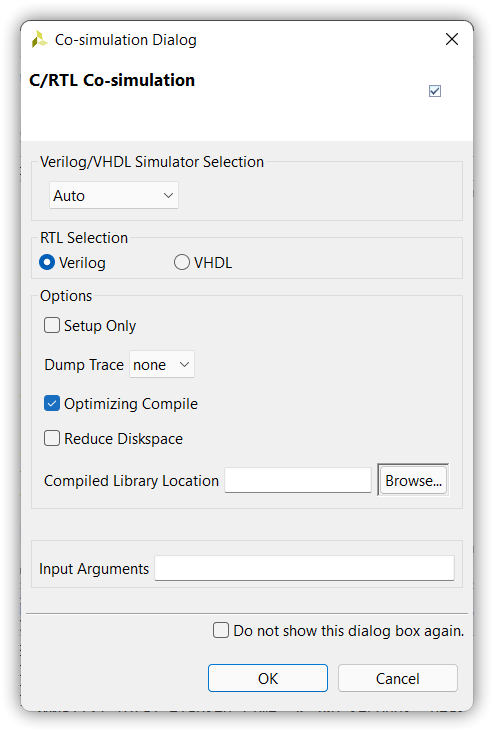
\includegraphics[width=.3\linewidth]{win/helloworld/C_RTL_cosim.png}
      \caption{CoSim 设置}
      \label{fig:C_RTL_cosim}
    \end{figure}

    此处,我们选择基于 Verilog 的 RTL 综合(也可以选择 VHDL),并且勾选优化编译与之前 CSim 一致。
    类似地,这里也可以设置对应的 Input Arguments。
    \begin{tip}[Linux 系统功能(仅限 Vivado 2017.4)]
      与 CSim 中类似,CoSim 也可以选择编译器为 GCC 或 Clang。(Ubuntu 20 上 CSim 可以通过,但是 CoSim 就会遇到 linker error。鉴于这些不确定性,不建议在 Linux 系统上展开这些工作,或严格按照 Vivado 支持的系统配置。)
    \end{tip}

    CoSim 的结果如\cref{fig:cosim_result} 所示,给出了 Verilog 测试的通过。
    如果代码更复杂,可以看到对应的 Latency 和 Interval 值。
    \begin{figure}[htbp]
      \centering
      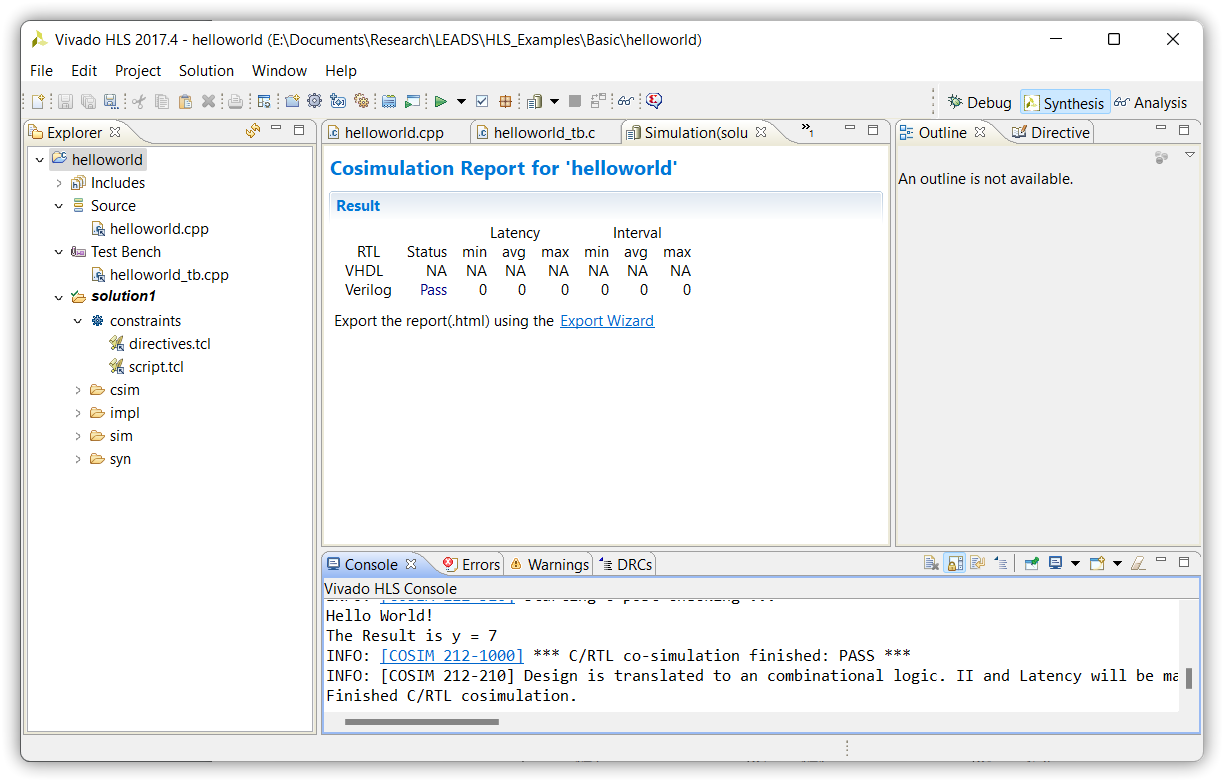
\includegraphics[width=.8\linewidth]{win/helloworld/cosim_result.png}
      \caption{CoSim 结果}
      \label{fig:cosim_result}
    \end{figure}

  \section{Exp --- 导出 IP 核}\index{Exp}

    在通过 CoSim 后,基本可以认定设计正确了,
    此时可以导出 IP 核(当然可以在窗口中设置为其他形式),
    点击 CoSim 右侧“棕色上有十字”的图标(Vitis 2021.2 为绿色箭头下拉框 Export),跳出\cref{fig:export_IP} 窗口进行设置。
    \begin{figure}[htbp]
      \centering
      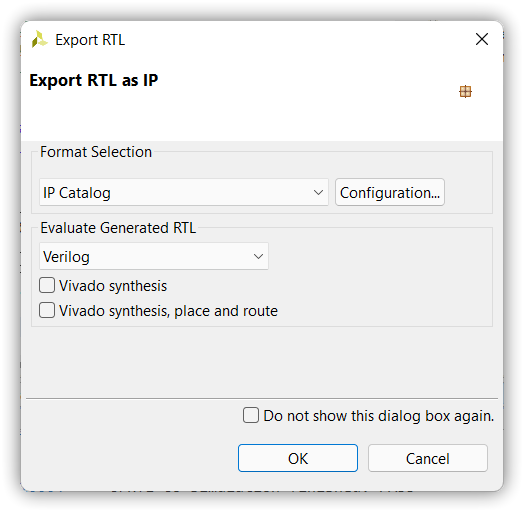
\includegraphics[width=.3\linewidth]{win/helloworld/export_IP.png}
      \caption{导出设置}
      \label{fig:export_IP}
    \end{figure}
    \begin{tip}[Vivado HLS Bug]
      此处会提示导出失败。而错误的原因实际上是 Xilinx Vivado 的一个 bug。
      Bug 的主要原因是 HLS 定义的 \texttt{ip\_version} 采用格式 \texttt{YYMMDDHHMM} 是一个有符号 32 位数,
      因此从2022年1月1日起均会导出失败。
      需要在 \href{https://support.xilinx.com/s/article/76960?language=en_US}{Xilinx 网站}下载对应的补丁,
      然后根据要求运行对应的 Python 代码修复问题。
    \end{tip}
    
    完成之后,我们就可以在 \texttt{impl/ip} 文件夹下找到生成的 zip 压缩的 IP 核。
    \texttt{impl} 文件夹下还会提供原始的 Verilog 代码,根据 Xilinx 官方描述,那些代码进攻测试使用,不代表最后导出的结果。

  \section{测试导出的 IP 核}

    \subsection{导入 IP 核}

      现在已经完成了所有的 HLS 设计工作,不过仍然可以验证我们导出的 \texttt{helloworld} IP 核的效果。
      在 IP Catalog 中新增 Repository,文件夹中加入解压后的 IP 核,得到如\cref{fig:manage_ip} 的效果。
      \begin{figure}[htbp]
        \centering
        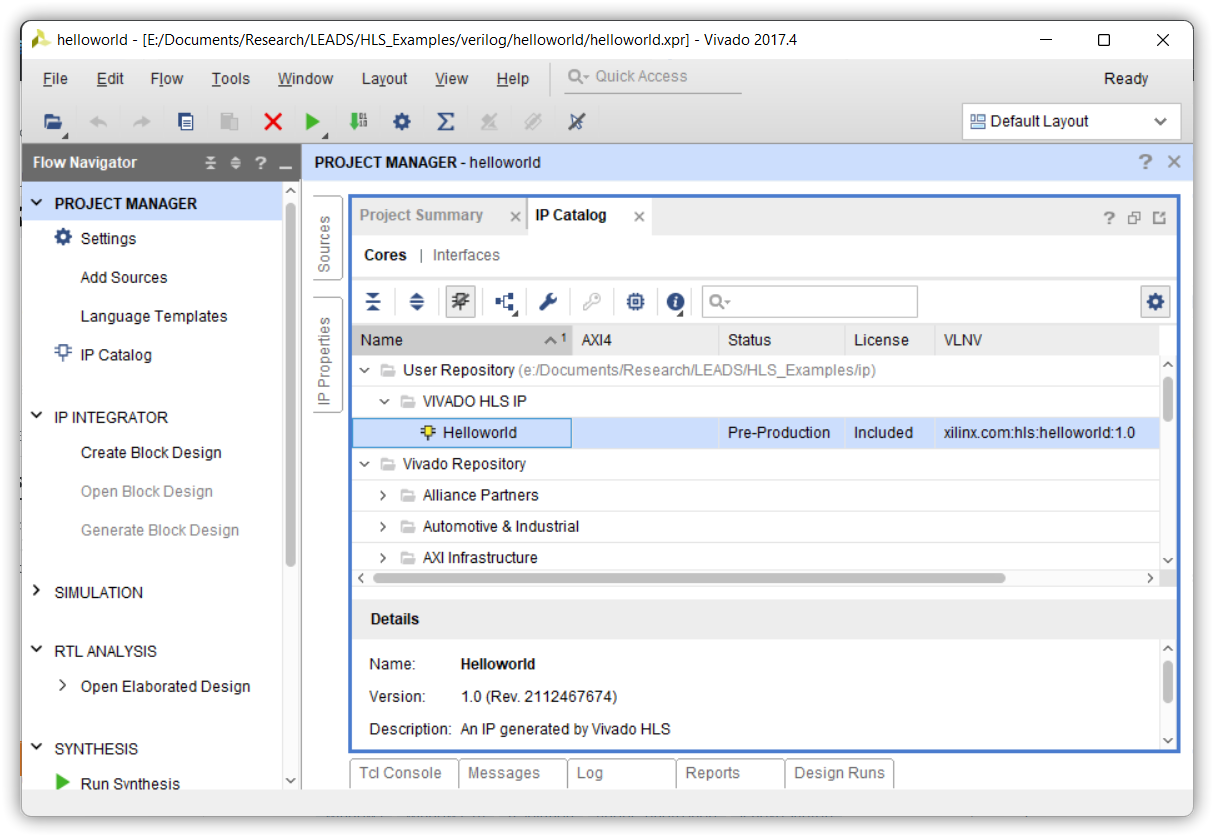
\includegraphics[width=.8\linewidth]{win/helloworld/manage_ip.png}
        \caption{管理 IP 核}
        \label{fig:manage_ip}
      \end{figure}

      双击使用 IP 核,并复制其中的 template 内容进入下一部分需要完成的 Test Bench 文件。

    \subsection{Test Bench 测试}


      增加 Test Bench 文件 \texttt{helloworld\_ip\_tb.v},模块名为 \texttt{HELLOWORLD\_IP\_TB}。
      其中创建的 \texttt{HELLO\_WORLD} instance 名为 \texttt{Uhelloworld}。
      展开 IP 内容可以看到 Insantiation Template,其中 \texttt{.veo} 文件给出了实例化的模板。
      \begin{lstlisting}[style={v}, title={helloworld\_ip\_tb.v}]
`timescale 1ns / 1ps

module HELLOWORLD_IP_TB();

    parameter   CYC         = 10;
    parameter   DELAY       = 1;
    parameter   START_TIME  = CYC;
    parameter   FINISH_TIME = 40 * CYC;
    reg         Clk = 0;

    // Input
    reg         Start       = 0;
    reg  [31:0] Data_in     = 0;
    // Output
    wire        Vld;
    wire [31:0] Data_out;
        
    HELLO_WORLD Uhelloworld (
        .b_ap_vld (Vld     ),  // output wire b_ap_vld
        .ap_start (Start   ),  // input wire ap_start
        .ap_done  (        ),  // output wire ap_done
        .ap_idle  (        ),  // output wire ap_idle
        .ap_ready (        ),  // output wire ap_ready
        .a        (Data_in ),  // input wire [31 : 0] a
        .b        (Data_out)   // output wire [31 : 0] b
    );

    initial begin
        #START_TIME  Start <= 1'b1;
        #FINISH_TIME $finish;
    end
    
    always #CYC Clk = ~Clk;
    
    always @(posedge Clk) begin
        #DELAY Data_in = Data_in + 1;    // increment one each clock
        #DELAY $display("Data Out: %b", Data_out); // display result
    end
    
endmodule // of HELLOWORLD_IP_TB
      \end{lstlisting}

      行为测试的结果如\cref{fig:behavioral_sim} 所示,
      这与我们设计的 \texttt{helloworld} 模块逻辑右移一位的目标相符合。
      \begin{figure}[htbp]
        \centering
        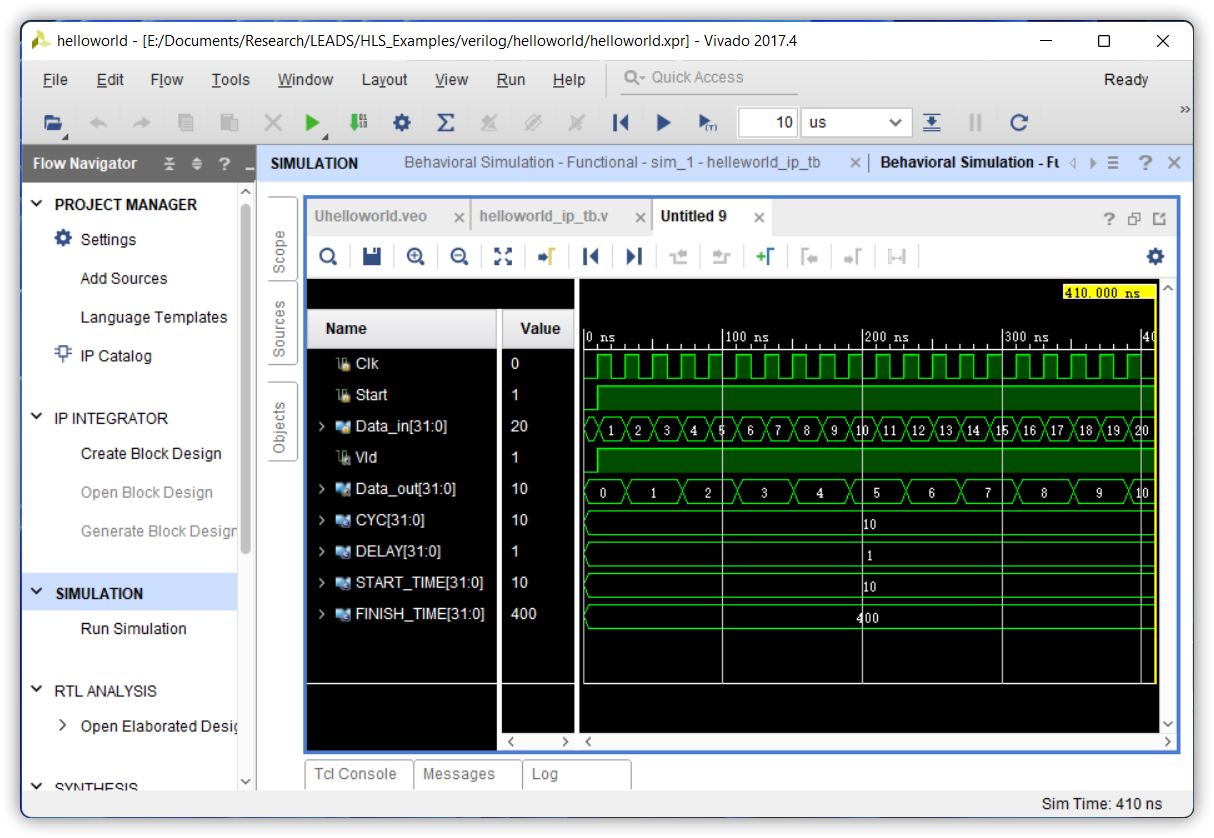
\includegraphics[width=.8\linewidth]{win/helloworld/behavioral_sim.png}
        \caption{行为仿真测试}
        \label{fig:behavioral_sim}
      \end{figure}

      我们也可以对其做 RTL 级分析,如\cref{fig:RTL_result} 所示。
      \begin{figure}[htbp]
        \centering
        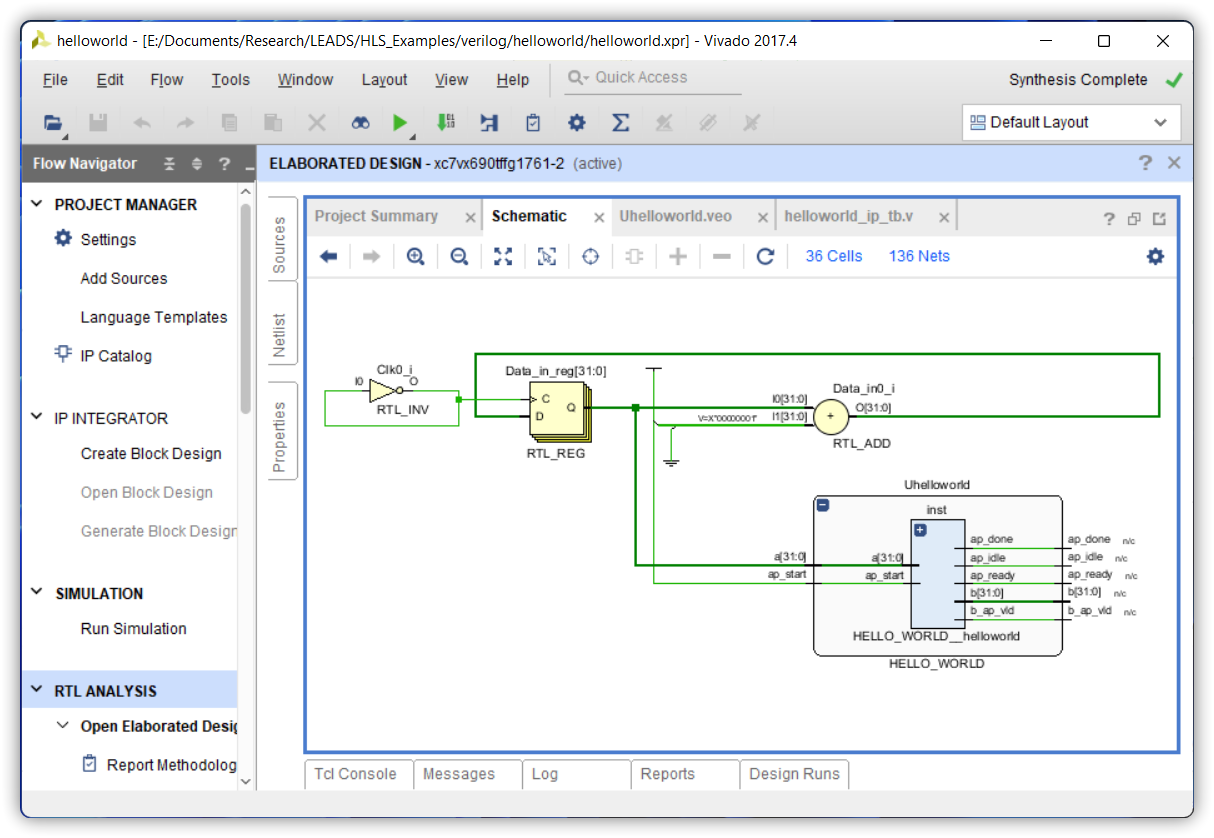
\includegraphics[width=.8\linewidth]{win/helloworld/RTL_result.png}
        \caption{RTL 级电路}
        \label{fig:RTL_result}
      \end{figure}

  \section{总结}

    在这个 Hello World 示例中,我们完整走完了从 C++ 代码生成 Verilog IP 核再验证 IP 核的过程,
    不过目前我们会发现如下的几个问题和局限,将在之后详细介绍:
    \begin{itemize}
      \item 使用了 C++ 自带的数据类型,其位数固定,例如 \texttt{int} 变量为 32 位,可能存在一定的浪费;
      \item 时序和并行度目前没有进行设计;
      \item 更加复杂的 C++ 不一定能够支持(编译器标准问题和 Syn 支持的语法)以及 HLS 工具额外提供的 C++ 库。
    \end{itemize}

\chapter{FFT}\index{FFT}

  \section{案例目标}

    快速傅立叶变换(fast Fourier transform,FFT)可以算是硬件设计的入门模块,
    此处用这个经典例子探讨 HLS 设计中的众多细节。
    在这个例子中,我们将实现:
    \begin{itemize}
      \item \DNF<完成后添加 FFT 示例实现的内容>
    \end{itemize}

  \section{FFT Naive}

    \subsection{设计架构}

      此处我们首先实践一个简单的 FFT 例子,其架构如\cref{fig:DIT-FFT-butterfly} 所示。
      \begin{figure}[htbp]
        \centering
        % https://en.wikipedia.org/wiki/File:DIT-FFT-butterfly.svg

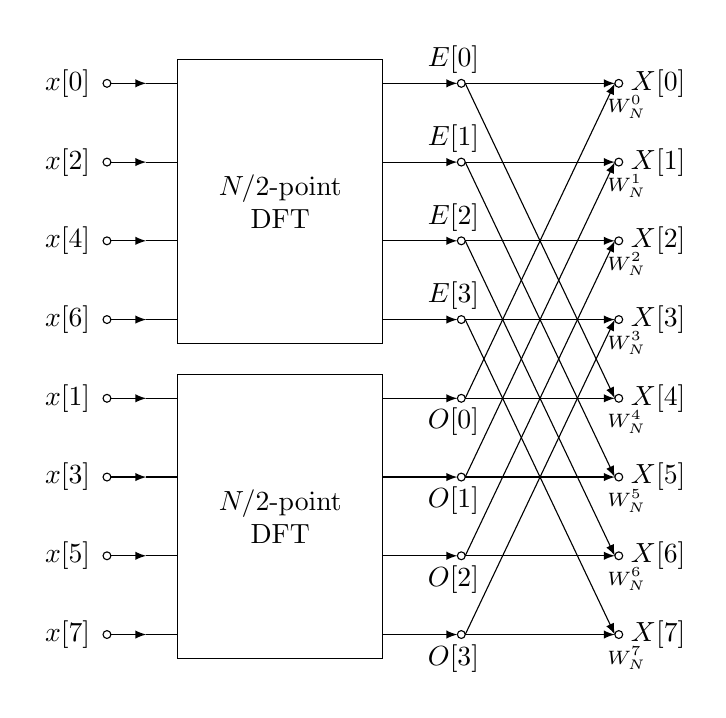
\begin{tikzpicture}% Example:
  \draw[fill=white, draw=white] (-0.5, 0.7) rectangle (8, -7.7); 
  \draw (0,0) node {$x[0]$};
  \draw (0,-1) node {$x[2]$} ;
  \draw (0,-2) node {$x[4]$} ;
  \draw (0,-3) node {$x[6]$} ;

  \draw (0,-4) node {$x[1]$} ;
  \draw (0,-5) node {$x[3]$} ;
  \draw (0,-6) node {$x[5]$} ;
  \draw (0,-7) node {$x[7]$} ;

  % arrow on the right of x's
  \foreach \n in {0,...,7} {
    \draw (0.5,-\n) circle(0.05)[fill=white]; 
    \draw [-latex] (0.55,-\n) -- (1, -\n); 
    \draw (1, -\n) -- (1.4, -\n); 
  }

  % blocks
  \draw(1.4, 0.3) rectangle (4, -3.3); 
  \draw(1.4, -3.7) rectangle (4, -7.3); 
  \draw(2.7, -1.5) node[text centered, text width=2cm] {$N/2$-point DFT};
  \draw(2.7, -5.5) node[text centered, text width=2cm] {$N/2$-point DFT};

  % E's and O's 
  \foreach \n in {0,...,7} {
    \draw [-latex] (4,-\n) -- (4.95, -\n); 
    \draw (5,-\n) circle(0.05)[fill=white]; 
  }
  \foreach \n in {0,...,3} {
    \draw (4.9,-\n + 0.3) node {$E[\n]$};
  }
  \foreach \n in {0,...,3} {
    \draw (4.9,-\n - 4 - 0.3) node {$O[\n]$};
  }

  % X's 
  \foreach \n in {0,...,7} {
    \draw (7,-\n) circle(0.05)[fill=white]; 
    \draw (7.5,-\n) node {$X[\n]$};
  }

  % Connecting X and E
  \foreach \n in {0,...,7} {
    \draw [-latex] (5.05, -\n) -- (6.95, -\n);
  }
  \foreach \n in {0,...,3} {
    \draw [-latex] (5.05, -\n) -- (6.95, -\n - 4);
  }
  \foreach \n in {0,...,3} {
    \draw [-latex] (5.05, -\n-4) -- (6.95, -\n);
  }

  % W's
  \foreach \n in {0,...,7} {
    \draw (7.1,-\n - 0.3) node {\scriptsize $W_N^{\n}$};
  }
\end{tikzpicture}

        \caption{蝶形 8点基2的 FFT 架构示意图~\copyright~[2022]~Yangwenbo99 at \href{https://en.wikipedia.org/wiki/File:DIT-FFT-butterfly.svg}{Wikipedia}}
        \label{fig:DIT-FFT-butterfly}
      \end{figure}

    \subsection{基本变量}

      \begin{warning}
        由于 Vivado 2017.4 中 HLS 编译器限制原因,无法使用最常用的 C++11 标准编写代码,此处我们会另外给出 C++98 的版本。
        此外代码的格式、标准库的使用均建议按照本文档的规范进行。
      \end{warning}

      从这里开始,我们心中需要有一个目标,就是\textbf{尽可能优化硬件的实现效果},
      而不是简单的写出一个正确的 C++ 代码。
      由于这不是正常的 C++ 代码写作,而是通过 HLS 工具,
      因此我们不是面向现代 C++ 编译器,而是面向 HLS 的高效综合,
      在许多习惯上我们要从一开始树立,这里给出了使用的 C++ 变量定义。

      \begin{definition}[整数类型]\index{ZZzhengshuleixing@整数类型}
        整数(integer)类型包括有符号(signed)和无符号(unsigned)两种。
        除去使用 C++ 中定义的 \indexint{char}\texttt{char}、\indexint{short}\texttt{short}、\indexint{int}\texttt{int}、\indexint{long}\texttt{long}、\indexint{long~long}\texttt{long long} 及其 \indexint{unsigned}\texttt{unsigned} 版本变量外,建议在涉及硬件实现的位数时使用 HLS 工具提供的 \indexint{ap\_int}\texttt{ap\_int} 和 \indexint{ap\_uint}\texttt{ap\_uint}。
        这些类型可以自由定义其位数,详见 \UGvitis{182} \UGvitis{578--599} \UGvivado{80} \UGvivado{218}。
      \end{definition}
      \begin{example}[整数类型]
        使用 HLS 定义的这些整数类型需要首先添加库。
        \begin{lstlisting}[language=C++,numbers=none]
#include <ap_int.h> // for type ap_int and ap_uint
        \end{lstlisting}
        然后,我们就可以给出如下定义的例子:
        \begin{lstlisting}[language=C++,numbers=none,morekeywords={ap\_int,ap\_uint}]
ap_int<12> a;             // 12-bit signed value 
ap_uint<8> b;             // 8-bit unsigned value
const int WIDTH = 4;      // define width (NOTE: const is required)
ap_uint<WIDTH> c;         // 4-bit unsigned value
typedef ap_int<6> TYPE_T; // TYPE_T is alias for ap_int<6>
TYPE_T d;                 // 6-bit signed value
        \end{lstlisting}
        在上述例子中,我们可以看到不同的整数变量定义方法,其中比较推荐定义一个常量类型的整数代指位数,
        并且在整个设计中主要用到的类型使用 \texttt{typedef} 定义。
        这样两种方法都可以减少代码中的错误以及降低修改的成本,使得代码更加整洁有条理。

        另外,默认的最大宽度是1024比特,如果需要更宽的数值(例如 4096),需要在 \verb|#include<ap_int.h>| 之前添加 \indextt{AP\_INT\_MAX\_W}\texttt{AP\_INT\_MAX\_W}
        \begin{lstlisting}[language=C++,numbers=none]
#define AP_INT_MAX_W 4096
        \end{lstlisting}
      \end{example}

      Vitis/Vivado HLS 中非常重要的是其固定位宽的浮点数类型,
      这在硬件设计中是非常重要的一环。
      \begin{definition}[浮点类型]\index{FZfudianleixing@浮点类型}
        浮点类型(float)包括了 C++ 中已有的 \indexfloat{double}\indextt{double}\texttt{double} 和 \indexfloat{float}\texttt{float} 类型(\UGvitis{186} \UGvitis{575--576} \UGvivado{186} \UGvivado{218})
        Vitis/Vivado 也提供了16位的半精度浮点数(half-precision floating-point data types) \indexfloat{half}\texttt{half} (\UGvivado{83--84})。
        不过最常用的是指定精度的浮点数类型(arbitrary precision fixed-point data types)\indexfloat{ap\_fixed}\texttt{ap\_fixed} 和 \indexfloat{ap\_ufixed}\texttt{ap\_ufixed},具体的内容可以参考 \UGvitis{183--184}\UGvitis{577-578} \UGvivado{81--82} \UGvivado{221--225}。
      \end{definition}
      
      \begin{example}[浮点类型]
        首先,类似整数类型,需要添加对应的头文件
        \begin{lstlisting}[language=C++,numbers=none]
#include <ap_fixed.h> // for type ap_fixed and ap_ufixed
        \end{lstlisting}
        然后,我们给出简单的使用例子,其他更加复杂的运用可以参考 UG 上的介绍和例子。
      \end{example}
      
      下面我们通过这个简单的例子来了解这些基本变量类型的使用。
      \begin{lstlisting}[language=C++,morekeywords={ap\_int,ap\_fixed,ap\_ufixed,std,cout,endl,to\_string}]
#include <iostream>
#include <ap_int.h>
#include <ap_fixed.h>

int main() {
    std::cout << "Compiler Version: " __VERSION__ << std::endl;

    /***** Integer *****/
    ap_int<4> i1 = 2;
    std::cout << "i1 = " << i1 << std::endl;
    i1 = 0b0101; // 5
    std::cout << "i1 = " << i1 << std::endl;
    i1 *= 2; // -6 (overflow)
    std::cout << "i1 = " << i1 << std::endl;
    i1 >>= 1; // -3 (right shift 1)
    std::cout << "i1 = " << i1 << std::endl;
    // convert to a binary string
    std::cout << "i1 = " << i1.to_string(2) << std::endl;
    // access the element at location 1
    std::cout << "i1[1] = " << i1[1] << std::endl;

    /***** Float *****/
    ap_fixed<6, 4> f1 = 3.1415926; // 3
    // 6 bits data, 4 bits before left of the binary point
    // therefore 1 sign, 3 int, 2
    std::cout << "f1 = " << f1 << std::endl;
    ap_fixed<6, 4> f2 = 5.99; // 5.75
    // the default behavior, truncation to minus infinity
    std::cout << "f2 = " << f2 << std::endl;
    ap_fixed<6, 4, AP_RND> f3 = 5.99;
    // round to plus infinity
    std::cout << "f3 = " << f3 << std::endl;
    f3 += ap_fixed<6, 4>(3.3); // -6.75 (overflow)
    std::cout << "f3 = " << f3 << std::endl;
    ap_ufixed<6, 4> f4 = 12.34; // 12.25
    std::cout << "f4 = " << f4 << std::endl;
    f4 += 4; // 0.25 (overflow)
    std::cout << "f4 = " << f4 << std::endl;

    return 0;
}
      \end{lstlisting}
      首先在第6行输出了编译器的版本,
      如果在 Vitis 2021.2 上我们可以看到 \texttt{6.2.0} 的输出。

      第9行定义了有符号整数类型变量 \texttt{i1},设定其初始值为 \texttt{2}。
      输出一个 \texttt{ap\_(u)int} 或 \texttt{ap\_(u)fixed} 变量可以直接使用 C++ 标准的输出流。
      第11行的赋值采用了 C++ 的标准方式,
      \texttt{0b} 表示二进制,
      \texttt{0x} 或 \texttt{0X} 表示十六进制等。
      第13行将数字乘二,由于四位有符号数范围为 \texttt{-8} 到 \texttt{7},
      这里产生了 overflow,由于采用补码的形式,所以得到的结果是 \texttt{-6}。
      第15行对数值进行了右移操作,需要注意这里是\textbf{算数右移},
      符合数学的运算规则和标准 C++ 的运算方式,因此输出结果为 \texttt{-3}。
      \begin{tip}[C++常数前缀]
        需要注意,二进制数的常数 \texttt{0b} 前缀在 C++14中才提供了支持,所以使用 Vivado 2017.4 的时候需要避免这样的运用。
        可以参考 \href{https://en.cppreference.com/w/cpp/language/integer_literal}{integer literal} 的介绍。
      \end{tip}

    \subsection{变量运算}

\part{实战演练}
\parttext{在了解了 Vitis HLS 的基本使用方法和设计思路之后,我们继续从 LEADS 课题组中具体 HLS 设计项目来进一步体会 HLS Design 的艺术。}

\chapter{均匀量化有限位宽下的实数矩阵乘法器}

\printindex

\end{document}
\endinput
